\documentclass[titlepage]{article}
\usepackage{graphicx}
\usepackage{listings}
\usepackage{color}
\usepackage[dvipsnames]{xcolor}
\usepackage{gensymb}
\usepackage[linguistics]{forest}
\usepackage{amsmath}
\usepackage{listings}
\usepackage{tikz}
\usetikzlibrary{mindmap}
\pagestyle{empty}

\definecolor{dkgreen}{rgb}{0,0.6,0}
\definecolor{gray}{rgb}{0.5,0.5,0.5}
\definecolor{mauve}{rgb}{0.58,0,0.82}
\definecolor{magenta}{HTML}{F10088}
\definecolor{plum}{HTML}{95298A}
\definecolor{tan}{HTML}{DC9C7B}
\definecolor{aquamarine}{HTML}{00B5BC}
\makeatletter
\setlength{\@fptop}{0pt}
\makeatother

\makeatletter
\newcommand*{\rom}[1]{\expandafter\@slowromancap\romannumeral #1@}
\makeatother

\lstset{frame=tb,
  language=Java,
  aboveskip=3mm,
  belowskip=3mm,
  showstringspaces=false,
  columns=flexible,
  basicstyle={\small\ttfamily},
  numbers=none,
  numberstyle=\tiny\color{gray},
  keywordstyle=\color{blue},
  commentstyle=\color{dkgreen},
  stringstyle=\color{mauve},
  breaklines=true,
  breakatwhitespace=true,
  tabsize=3
}

\title{ECE408 - Applied Parallel Programming \\ Final Report}
\author{Neil Singh (ngsingh2) \\ Patrick McMahon (pfmcmah2) \\ Matthew Krikorian (krikorn2)}

\begin{document}

\maketitle

\section*{Milestone 1}
Milestone 1 of this project was mostly setting up our test environment and preparing it to start developing the later parts of this project. 

\subsection*{Running Time of m1.1.py}
For m1.1.py, we had an accuracy of 0.8673, and an elapsed running time of 9.76 seconds.

\subsection*{Running Time of m1.2.py}
For m1.2.py, we had an accuracy of 0.8673, and an elapsed running time of 3.19 seconds.

\subsection*{Most Time Consuming Kernels}
Some of the most time consuming kernels when running the nvprof profile were the\textit{implicit\_convolve\_sgemm} kernel, taking up 36.96\% of the execution time, the \textit{activation\_fw\_4d\_kernel} kernel, taking up 14.33\% of the execution time, and the \textit{pooling\_fw\_4d\_kernel} kernel, which took up 10.69\% of the programs execution time.

\newpage

\section*{Milestone 2}
In this milestone of the project, we were tasked with writing sequential convolution code. Using the skeleton from our textbook, and the corresponding data accesses, we successfully implemented the function below.

\begin{figure}[h!]
\begin{lstlisting}[language=C++]
{
    const int B = x.shape_[0];
    const int M = y.shape_[1];
    const int C = x.shape_[1];
    const int H = x.shape_[2];
    const int W = x.shape_[3];
    const int K = k.shape_[3];

    int H_out = H - K + 1;
    int W_out = W - K + 1;

    for (int b = 0; b < B; ++b)
    {
      for (int m = 0; m < M; m++)
      {
        for (int h = 0; h < H_out; h++)
        {
          for (int w = 0; w < W_out; w++)
          {
            y[b][m][h][w] = 0;

            for (int c = 0; c < C; c++)
            {
              for (int p = 0; p < K; p++)
              {
                for (int q = 0; q < K; q++)
                {
                  y[b][m][h][w] += x[b][c][h + p][w + q] * k[m][c][p][q];
                }
              }
            }
          }
        }
      }
    }
}
\end{lstlisting}
\caption{Our CPU implementation of the convolutional layer in MxNet}
\end{figure}

\newpage

\subsection*{Our Results For Respective Models}

\begin{figure}[h!]
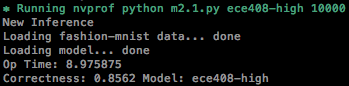
\includegraphics[width=\linewidth]{ece-408-high-10000.png}
\caption{Accuracy and elapsed time for high correctness and sample size 10000}
\label{fig:flowFree}
\end{figure}

\begin{figure}[h!]
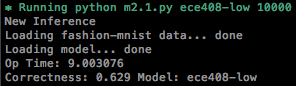
\includegraphics[width=\linewidth]{ece-408-low-10000.png}
\caption{Accuracy and elapsed time for low correctness and sample size 10000}
\label{fig:flowFree}
\end{figure}

\newpage
\section*{Milestone 3}
In this milestone we were tasked with writing a baseline paralllel convolution kernel that had to pass several baseline tests. This implementation is very sub-optimal, as it uses a TILE\_WIDTH of 1.
\begin{figure}[h!]
\begin{lstlisting}[language=C++]
{
    const int H_out = H - K + 1;
    const int W_out = W - K + 1;
    
    #define y4d(i3,i2,i1,i0) y[(i3) * (M * H_out * W_out) + (i2)*(H_out * W_out) + (i1)*(W_out) + i0]
    #define x4d(i3,i2,i1,i0) x[(i3) * (C * H * W) + (i2)*(H * W) + (i1)*(W) + i0]
    #define k4d(i3,i2,i1,i0) k[(i3) * (C * K * K) + (i2)*(K * K) + (i1)*(K) + i0]

    int W_grid = ceil(W_out / (float)TILE_WIDTH);
    int H_grid = ceil(H_out / (float)TILE_WIDTH);
    int n, m, h, w, c, p, q;
    n = blockIdx.x;
    m = blockIdx.y;
    h = blockIdx.z / W_grid + threadIdx.y;
    w = blockIdx.z % W_grid + threadIdx.x;
    
    float acc = 0;
    for (c = 0; c < C; c++) {
        for (p = 0; p < K; p++) {
            for (q = 0; q < K; q++) {
                if (h+p < H && w+q < W)
                    acc += x4d(n, c, h+p, w+q) * k4d(m, c, p, q);
            }
        }
    }
    y4d(n, m, h, w) = acc;

    #undef y4d
    #undef x4d
    #undef k4d
}
\end{lstlisting}
\caption{Our GPU implementation of the convolutional layer in MxNet}
\end{figure}

\newpage
\subsection*{Nvprof GPU Profile}
\begin{figure}[h!]
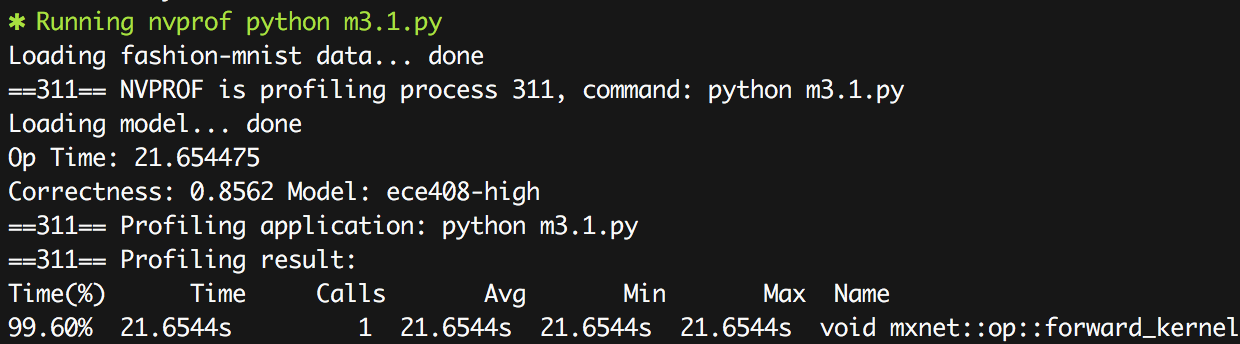
\includegraphics[width=\linewidth]{nvprof.png}
\caption{Nvprof GPU profile for our forward kernel}
\label{fig:flowFree}
\end{figure}


\section*{Team Contributions}
We all met up together and finished the sequential code for the convolutional layer in person. We also met up and wrote the parallel code together after meeting up in person, as well as crafting this report together for submission.

\end{document}















